\documentclass[a5paper,10pt]{ltjsarticle}
\usepackage[margin=13mm,bottom=16mm]{geometry}
\usepackage{luatexja-fontspec,amsmath,amssymb,graphicx,tikz,fancyhdr}
\usepackage[hidelinks]{hyperref}
\setmainjfont{BIZ UDGothic}
\setlength{\parindent}{0pt}\setlength{\parskip}{5pt}
\pagestyle{fancy}\fancyhf{}\fancyfoot[L]{\small LinearKnot　機内補講}\fancyfoot[R]{\thepage\,/\,12}
\renewcommand{\headrulewidth}{0pt}
\newcommand{\unit}[2]{\clearpage{\small 動画①　#1}\par{\Large\bfseries #2}\par\medskip}
\newcommand{\task}[1]{\par\medskip\textbf{紙で確かめる}\quad #1}
\newcommand{\ans}[1]{\par\textbf{照合}\quad #1}
\begin{document}
{\small LinearKnot　機内用テキスト／2026年11月27日版}\par\bigskip
{\LARGE\bfseries Outside はなぜ\\backprop なのか}\par\medskip
RNA の塩基対確率を、分配関数の計算グラフから手で導く。紙では $\alpha$ を実数の inside、$\beta$ を実数の outside と書く。動画①は「アニメーション版」（33分50秒）を使う。
\par\medskip
\begin{tabular}{@{}ll@{}}
紙面 & 動画①の再生位置と問い\\
2--3 & 00:00／03:10　途中の値を通る微分とは？\\
4--5 & 08:39／10:09　木を切ると何が残るか？\\
6 & 16:34　1本の path でも同じ式か？\\
7--8 & 20:29／24:33　出現回数と確率の違いは？\\
9 & 11:41／14:59　穴のある BE を微分できるか？\\
10 & 27:05　塩基対に印を付けるには？\\
11--12 & 30:10　枝刈り後の微分と仕上げの演習
\end{tabular}
\par\bigskip
\textbf{最初に解いてみる。} 二つの部分問題の値が2と3。それらを同時に使う規則の重みが4。別の規則は重み6だけを加える。全体の重みはいくつか。左の部分問題の値を0.01増やすと全体はいくつ増えるか。この2問に同じ計算図で答えるのが本書の出発点である。
\par\medskip
動画は機内に入る前に MP4 を端末へ保存する。紙面はオフラインで完結する。\href{https://youtu.be/kzB3MKkpCCY}{動画①　\texttt{youtu.be/kzB3MKkpCCY}}
\unit{00:00／03:10}{入力・途中の値・出力}
計算グラフとは、ある値をどの値から計算したかを矢印で示した図である。入力を $x$、途中の値を $u=x+1$、出力を $v=4u$ と定義する。
\begin{center}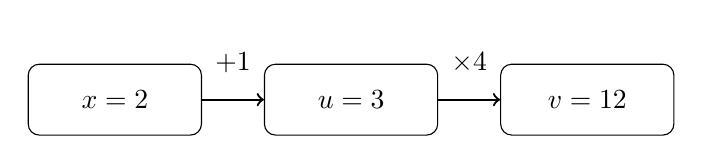
\begin{tikzpicture}[every node/.style={draw,rounded corners,minimum width=22mm,minimum height=9mm}]
\node(a) at (0,0){$x=2$};\node(b) at (3,0){$u=3$};\node(c) at (6,0){$v=12$};
\draw[->,thick](a)--node[above,draw=none]{$+1$}(b);\draw[->,thick](b)--node[above,draw=none]{$\times4$}(c);
\end{tikzpicture}\end{center}
順方向では、左から右へ値を計算する。逆方向では、各頂点 $q$ に「$q$ を少し変えたとき出力 $v$ がどれだけ変わるか」すなわち $\bar q=\partial v/\partial q$ を書く。
\[
\bar v=1,\qquad \bar u=\bar v\frac{\partial v}{\partial u}=4,
\qquad \bar x=\bar u\frac{\partial u}{\partial x}=4.
\]
これは連鎖律を出力から入力へ順に適用したもの。多くの途中の値について、1回の逆向きの走査でこの微分を得る計算法を逆モード自動微分（backprop）という。
\task{$x=2.01$ に置き換え、実際の変化を表に書こう。どの段階で変化量が4倍になるか。}
\ans{$u=3.01,\ v=12.04$。入力の変化 $0.01$ は足し算では保存され、最後の掛け算で $0.04$ になる。}
\unit{03:10 の次の画面}{分岐したら、戻る寄与を足す}
入力を $x=3$ とし、二つの途中の値を $a=3x,\ b=2x$、出力を $y=a+b$ とする。両方の枝は同じ入力を読む。
\begin{center}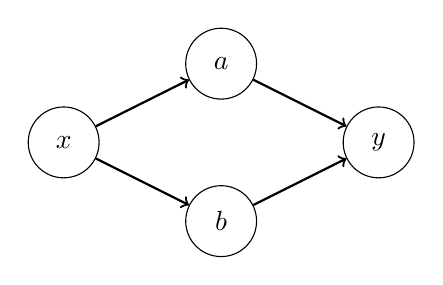
\begin{tikzpicture}[every node/.style={draw,circle,minimum size=9mm}]
\node(x)at(0,0){$x$};\node(a)at(2,1){$a$};\node(b)at(2,-1){$b$};\node(y)at(4,0){$y$};
\foreach \i/\j in {x/a,x/b,a/y,b/y}{\draw[->,thick](\i)--(\j);}
\end{tikzpicture}\end{center}
順方向は $a=9,b=6,y=15$。逆方向は $\bar y=1$ に始まり、和の各入力へ $\bar a=\bar b=1$ が届く。$x$ の場所では2本分を合わせる。
\[
\bar x=\bar a\,3+\bar b\,2=5.
\]
後から来た値で上書きすれば、一方の枝の寄与を失う。文法でも、一つの部分問題が異なる親や規則に使われるたびに寄与を加算する。
\task{出力を $y=a+2b$ に変えると、$\bar b,\bar x$ はいくつか。}
\ans{$\bar b=2$、$\bar x=1\cdot3+2\cdot2=7$。順方向の式 $y=7x$ でも確認できる。}
\unit{08:39}{Inside は導出木の重みの和}
導出木は、構造を組み立てる各段で規則を1つずつ選んだ記録である。局所重みとは、その規則をその位置で使うときに掛ける数。木の重みは全頂点の局所重みの積になる。項目 $p$（状態名と座標）を根とするすべての導出木の重みの和を $\alpha(p)$ とする。
\[
\alpha(p)=\sum_{e:\,p\leftarrow C_e} w_e\prod_{j=1}^{k_e}\alpha(c_j).
\]
$e$ は分割点を含めて具体化した規則、$w_e$ は局所重み、$C_e=(c_1,\ldots,c_{k_e})$ は順序付きの子の列。子が0個の積は1。全体の根を $r$ とすると分配関数は $Z=\alpha(r)$。
\par\textbf{紙面1の例。} $r$ が「重み4で子 $A,B$ を組み合わせる」か「重み6で終了する」かを選ぶ。$\alpha(A)=2,\ \alpha(B)=3$ なら
\[
Z=4\alpha(A)\alpha(B)+6=30.
\]
上の和は導出について取る。同じ構造を複数の導出が作る場合、その構造への寄与はそれらを合計する。
\task{子が $A$ だけの第3の規則（重み5）を加えると $Z$ は？}
\ans{$30+5\cdot2=40$。新しい規則は以前の2通りと同時には選ばないので、寄与を和に加える。}
\unit{10:09}{木に穴を空けると outside が残る}
\begin{center}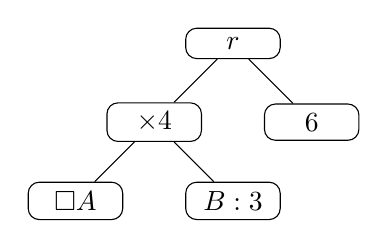
\begin{tikzpicture}[every node/.style={draw,rounded corners,minimum width=12mm}]
\node(r)at(0,2){$r$};\node(e)at(-1,1){$\times4$};\node(a)at(-2,0){$\square A$};\node(b)at(0,0){$B:3$};\node(f)at(1,1){$6$};
\foreach \i/\j in {r/e,r/f,e/a,e/b}{\draw(\i)--(\j);}
\end{tikzpicture}\end{center}
$A$ を選んだ位置で部分木を外す。残った文脈には、根で選んだ規則の4と、兄弟 $B$ の重みの和3が含まれる。$A$ を含まない選択肢6には穴を置けない。穴に任意の重み $t$ を入れると $Z(t)=12t+6$。穴の外が与える倍率は12である。
\[
\beta(A)=\frac{\partial Z}{\partial\alpha(A)}=12.
\]
一般に全体の根から $\beta(r)=1$ で始め、各規則 $e$ について親から子 $c_i$ の各出現に返す：
\[
\beta(c_i)\mathrel{+}=\beta(p)\,w_e\prod_{j\ne i}\alpha(c_j).
\]
親の倍率、規則の重み、他の子の重みを掛ける。この式は紙面4の積を $i$ 番目の入力で微分した式そのものである。親を先に逆走査すれば、その親に届いたすべての文脈が次の子に渡る。
\task{$A$ を0.01増やしたとき、$Z$ の変化は？}\ans{$12\times0.01=0.12$。}
\unit{16:34}{Forward–backward は子が1つの場合}
始点 $s$ から中継点 $A$ を経由して終点 $t$ に行く経路の重みを $2\times5$、中継点 $B$ を通る経路を $3\times7$ とする。各矢印の重みを掛け、経路全体では足す。
\[
Z=2\cdot5+3\cdot7=31.
\]
$\alpha(A)=2$ は $A$ までの経路重み、$\beta(A)=5$ はそこから終点までの重み。$A$ を通る確率は
\[
P(A)=\frac{\alpha(A)\beta(A)}{Z}=\frac{10}{31}.
\]
始点から $A$ への重みを $x$ と書き直すと $Z(x)=5x+21$。$\partial Z/\partial x=5$ は $A$ から先の係数と同じになる。木に戻れば、ある規則が2つの子を同時に必要とする。片方から見た「残り」には、根への経路に加えて兄弟の部分木も入る。これが紙面5の積である。
\task{$B$ を通る確率を出し、2つの確率の和を確かめよう。}\ans{$21/31$。この図では、どの経路も $A,B$ のちょうど一方を通るため和が1になる。任意の2項目に対して成り立つ正規化ではない。}
\unit{20:29／24:33}{出現回数と出現確率を区別する}
導出木 $T$ の重みを $w(T)$、そこに項目 $A$ が出現する回数を $N_A(T)$ とする。各出現に同じ印 $z$ を掛けると
\[
Z(z)=\sum_T w(T)z^{N_A(T)},\qquad
\frac{Z'(1)}{Z(1)}=\sum_T\frac{w(T)}{Z(1)}N_A(T).
\]
$Z(1)>0$ とする。右辺は平均出現回数。出現回数が0または1なら出現確率でもある。
\par\textbf{反例。} 根の規則が同じ子 $A$ を2回使い、$\alpha(A)=2$、規則の重みは1。他に規則がない場合 $Z=\alpha(A)^2=4$。左右の子の位置を区別して微分すると
\[
\beta(A)=\alpha(A)+\alpha(A)=4,\qquad
\alpha(A)\beta(A)/Z=2.
\]
少なくとも1回出る確率は1。それでも出現回数は2になる。計算グラフの一つの頂点が導出木の複数の位置から参照されるためである。
\task{「子の列」を集合に置き換えると、上の例では何を失うか。}\ans{同じ $A$ の2番目の出現が消え、順方向の積も逆方向の加算も変わる。}
\unit{24:33}{対数表で backprop すると何が返るか}
実装と旧教科書の多くの式は対数の表を使う。$a=\log\alpha(A)$、$\ell=\log Z$ とする。$Z>0,\ \alpha(A)>0$ の範囲で連鎖律を使うと
\[
\frac{\partial\ell}{\partial a}
=\underbrace{\frac{1}{Z}}_{\partial\ell/\partial Z}
\underbrace{\beta(A)}_{\partial Z/\partial\alpha(A)}
\underbrace{\alpha(A)}_{\partial\alpha(A)/\partial a}.
\]
したがって、実数の計算の出力 $Z$ を逆伝播すると実数 outside $\beta$、対数の出力 $\log Z$ を対数 inside まで逆伝播すると期待出現回数が得られる。教科書の log outside 表に保存する $\log\beta$ は、後者の微分とは別の量である。
\par\textbf{数値で照合。} 紙面5の $A$ について $\alpha=2,\beta=12,Z=30$。実数 outside は12、log outside は $\log12$、対数どうしの微分は $24/30=0.8$。
\task{兄弟の inside を0とした場合、子への寄与を「親の積÷注目する子の値」で計算して安全か。}\ans{注目する子が0なら $0/0$ が生じる。紙面5のように他の子だけを掛ければよい。$Z=1+5X$ なら $X=0$ でも $\partial Z/\partial X=5$。}
\unit{11:41／14:59}{BE の穴と「微分する穴」を分ける}
\begin{center}\includegraphics[width=.68\linewidth,height=38mm,keepaspectratio]{04_arc_case1.png}\end{center}
横軸は塩基位置。上の弧は固定対、下は追加対。20塩基例では $b=\mathrm{BE}(1,14;4,11)$ は $[1,4]\cup[11,14]$ の2本の腕を扱う。$u=\mathrm{WI}(5,5)$ が5番を、$v=\mathrm{VP}(6,17)$ がこの導出で $[6,10]\cup[15,17]$ を担当する。ここで $u,v$ は部分問題の名前である。
\[
\Delta\alpha(p)=w\alpha(b)\alpha(u)\alpha(v),\quad
\Delta\beta(b)=\beta(p)w\alpha(u)\alpha(v).
\]
BE の中央 $[5,10]$ は配列上の穴。一方、微分では計算グラフで $\alpha(b)$ という入力を丸ごと外す。兄弟の WI と VP が残るのはこのため。区間の枠が重なることと、同じ塩基対・局所エネルギーを重複して数えることは区別する。
\task{$\beta(p)=7,w=2,\alpha(u)=1,\alpha(v)=5$ と置くと？}
\ans{この規則から $b$ に70を加える。他の親からの寄与があればさらに足す。}
\unit{27:05}{一つの塩基対に印を置く}
位置 $i,j$ の塩基が対になるイベントを考える。各導出で対象の対をちょうど1回報告する規則に印 $z$ を掛ける。報告する規則の使用回数を $N_{ij}$ とすれば、紙面7の式がそのまま使える。
\[
P((i,j)\in T)=\frac{1}{Z}
\sum_{e\;\text{が対を報告}}\beta(p_e)w_e\prod_{c\in C_e}\alpha(c).
\]
$p_e$ は規則 $e$ の親。対を含む各導出に報告が1回、含まない導出に0回という条件が必要である。同じ対を親と子の両方で報告すれば期待報告回数を過大に数える。
\par\textbf{エネルギーとの対応。} $w_e=\exp[-E_e/(RT)]$ とし、温度 $T$ と気体定数 $R$ は固定する。$E_e$ がこの規則の1回ごとのエネルギーであれば、
\[
\frac{\partial\log Z}{\partial E_e}
=-\frac{\mathbb E[N_e]}{RT}.
\]
符号は負。規則のエネルギーを上げるほど、その規則を使う導出の重みは下がる。
\task{固定足場の対が全導出に必ず含まれ $Z>0$ なら、その対の確率は？}\ans{1。これは固定した足場を条件とする分布での値である。}
\unit{30:10}{有限 beam のグラフを固定する}
各段で一部の候補だけを残す方法を beam と呼ぶ。残った規則と項目が作る計算グラフを $H$ とすると、inside が実際に計算した値は
\[
Z_H=\sum_{T\;\text{が}\;H\;\text{内で導出可能}}w(T).
\]
同じ $H$ の規則を同じ重みで逆にたどれば、得られるのは $Z_H$ の微分である。順位の変化によって消した規則が復活する効果はこの微分に含まれない。逆走査で規則を再生成する実装でも、順方向で残した親・子・条件を一致させる必要がある。
\par\textbf{紙で実験。} 規則1の重みを $x$、規則2の重みを2とし、最大の候補を1つ残す。$x=3$ の周りでは $Z_H=x$。候補を両方使う exact では $Z=x+2$。
\[
P_H(1)=1,\qquad P_{\rm exact}(1)=3/5.
\]
\task{$x=1$ にして選び直した場合と、最初の候補を固定したままの場合の値は？}
\ans{選び直せば規則2が残り2。初めの $H$ のままなら1。切替点 $x=2$ では $\max(x,2)$ の通常の微分は定まらない。}
\unit{通覧後}{閉じて解く3問}
\textbf{問1　枝を1つ追加する。} 紙面4の $Z=4AB+6$ に $5A$ を加える。ここで $A,B$ は子の実数 inside で $A=2,B=3$。$Z,\beta(A)$、$A$ の出現確率を求めよ。各導出で $A$ は高々1回。
\par\textbf{問2　紙面9の規則。} 親の outside が7、重み2、子の inside は順に $(3,1,5)$。$u$ に返す値、親の inside に足す値を別々に求めよ。
\par\textbf{問3　何を微分したのか。} 紙面5の数値で $\log Z$ を実数 inside $A$ で微分せよ。次に $\log A$ で微分し、違いを説明せよ。
\par\medskip\hrule\medskip
\textbf{解1}\quad $Z=40,\ \beta(A)=4B+5=17$。$2\cdot17/40=0.85$。全列挙でも $A$ を使う2規則の重みは24と10。\\
\textbf{解2}\quad $u$ に $7\cdot2\cdot3\cdot5=210$。親に $2\cdot3\cdot1\cdot5=30$。\\
\textbf{解3}\quad $\partial\log Z/\partial A=12/30=0.4$。$\partial\log Z/\partial\log A=2\cdot0.4=0.8$。後者は、入力を相対的に変化させたときの感度である。
\par\medskip
\textbf{原典と続き}\quad Jason Eisner (2016), \emph{Inside-Outside and Forward-Backward Algorithms Are Just Backprop}, pp. 1--17. \href{https://aclanthology.org/W16-5901/}{doi:10.18653/v1/W16-5901}。LinearCParty 教科書第3巻第6章では、この原理を具体的な文法規則に展開する。動画の版に対応する教材ソースは LinearKnot の \texttt{docs/inside-outside-ja} ブランチにある。
\end{document}
